\documentclass[11pt,a4paper]{article}
\usepackage{fontspec}
\setmainfont{Lato}[Path=/usr/share/fonts/truetype/lato/,Extension=.ttf,UprightFont=*-Regular,BoldFont=*-Bold,ItalicFont=*-Italic,BoldItalicFont=*-BoldItalic]
\setmonofont{DejaVu Sans Mono}[Scale=0.8]
\usepackage[spanish]{babel}
\usepackage[margin=2cm]{geometry}
\usepackage{xcolor,enumitem,booktabs,array,graphicx}
\usepackage[hidelinks]{hyperref}
\graphicspath{{figuras/}}
% generado por pruebas/conftest.py: no editar a mano
\newcommand{\PruebasOk}{77}
\newcommand{\PruebasTotal}{81}
\newcommand{\PruebasFallan}{4}

\definecolor{verde}{HTML}{0B5D45}
\definecolor{gris}{HTML}{5C6D7E}
\setlength{\parindent}{0pt}
\setlength{\parskip}{5pt}
\newcommand{\seccion}[1]{\bigskip\par{\Large\bfseries\color{verde}#1}\par\smallskip\hrule\smallskip}
\newcommand{\sub}[1]{\medskip\par{\large\bfseries #1}\par}
\newcommand{\nota}[1]{{\small\color{gris}\itshape #1}\par}

\begin{document}

{\LARGE\bfseries\color{verde} Guía del tablero (dashboard)}\\[4pt]
{\large Cómo abrirlo, cómo leerlo y cómo demostrarlo en la exposición}\\[2pt]
{\color{gris}Angel Apolo · Fernando Terán · Stalyn Ochoa · Karla Barrera}

\seccion{1. Abrirlo}
El tablero es una página web que se sirve desde el propio computador. Solo necesita Python 3, sin librerías adicionales.

\begin{enumerate}[leftmargin=*]
\item Descomprimir el .zip y entrar a la carpeta \texttt{Proyecto\_Interciclo/v2}.
\item Abrir el tablero:
  \begin{itemize}
  \item \textbf{Windows:} doble clic en \texttt{abrir\_dashboard.bat}, o en una terminal: \texttt{python servir\_dashboard.py}
  \item \textbf{Linux o Mac:} \texttt{./abrir\_dashboard.sh}, o \texttt{python3 servir\_dashboard.py}
  \end{itemize}
\item Se abre solo en el navegador. Si no, entrar a \url{http://localhost:8097}.
\item Para cerrarlo, Ctrl+C en la terminal.
\end{enumerate}
\nota{No abrir \texttt{index.html} con doble clic: el navegador bloquea la carga de los datos desde un archivo local y aparece ``No se pudieron cargar los datos''. Siempre usar el servidor. Si el puerto 8097 está ocupado: \texttt{python servir\_dashboard.py 8098}.}

\seccion{2. Controles que comparten todas las secciones}
\begin{tabular}{@{}>{\bfseries}p{3.6cm}p{12.6cm}@{}}
Barra izquierda & Las seis secciones. Conviene seguir el orden de arriba hacia abajo. \\[3pt]
Reloj (arriba derecha) & Hora del día simulado. \textbf{Reproducir} avanza el día; −15 / +15 min saltan; el selector cambia la velocidad (2, 5 o 15 min por segundo). \\[3pt]
Línea de tiempo & Debajo del reloj. Clic o arrastre para ir a cualquier hora. Las marcas rojas y ámbar son los incidentes del día. \\[3pt]
Día simulado & Abajo a la izquierda: L M X J V S D, los 7 días de test (36 a 42). Cambia la ciudad y el detector; la ficha ``El día simulado'' dice qué lo caracteriza (lluvia, demanda, incidentes). La línea azul marca el día de lluvia. \\[3pt]
Fuente de datos & Abajo a la izquierda. \textbf{Sensores}: detectores que cuentan todos los autos. \textbf{V2X 50 \%}: solo la mitad de los autos, los conectados. Cambia todas las cifras y mapas. \\[3pt]
Guía turquesa & Arriba de cada sección: qué se está viendo y qué probar. Se cierra con la ×. \\[3pt]
Ayudas ``?'' & Pasar el mouse sobre el círculo: explicación corta de cada término técnico. \\
\end{tabular}

\seccion{3. Qué muestra cada sección}

\sub{Inicio}
Qué es el sistema en lenguaje simple, de dónde salen los datos, las tres cifras clave (predecir, detectar, avisar) con un botón para ir a cada una, y un glosario de doce términos.

\sub{Ciudad en vivo}
\begin{center}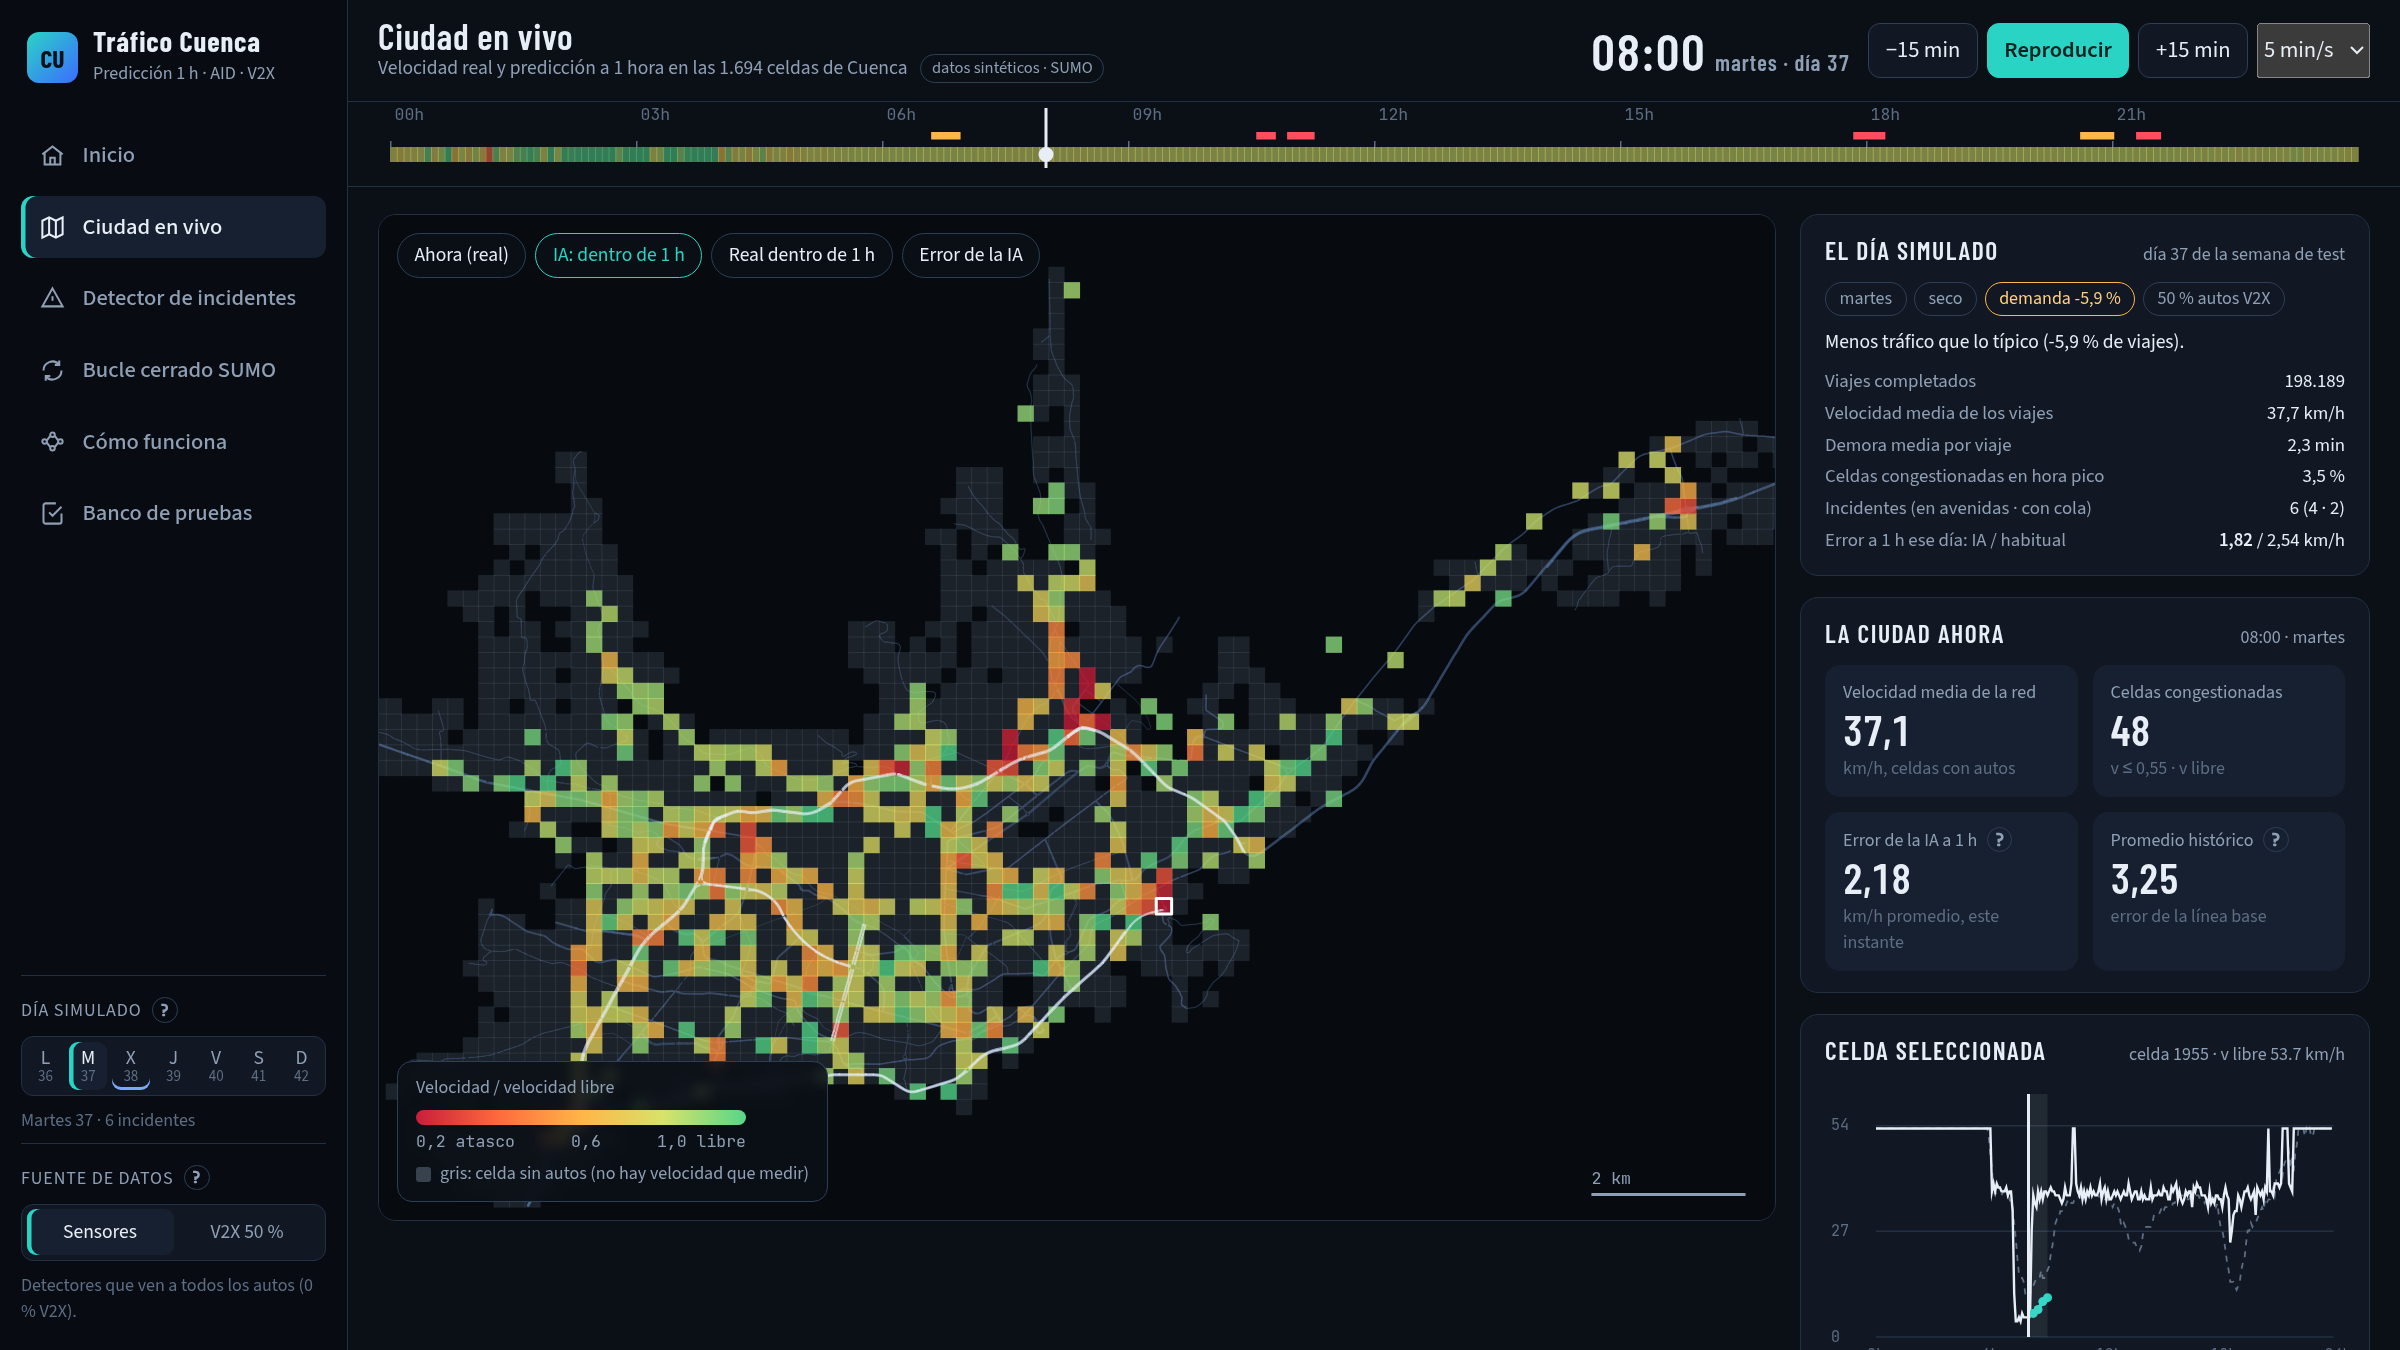
\includegraphics[width=.86\textwidth]{dash_ciudad_pred.png}\end{center}
Mapa de las 1694 celdas de 200~m, de verde (tráfico libre) a rojo (atasco). Las cuatro pastillas sobre el mapa cambian la capa:
\begin{itemize}[leftmargin=*]
\item \textbf{Ahora (real)}: el tráfico a la hora del reloj.
\item \textbf{IA: dentro de 1 h}: lo que la IA predice para una hora después.
\item \textbf{Real dentro de 1 h}: lo que de verdad pasó. Si se parece a la anterior, la IA acertó.
\item \textbf{Error de la IA}: solo las celdas con autos; gris si el error es menor a 2~km/h, rojo si predijo más lento, azul si más rápido.
\end{itemize}
Las celdas \textbf{grises} no tienen autos en ese momento: no hay velocidad que medir ni que predecir, así que no se colorean. Al hacer clic en una celda, la gráfica de la derecha muestra su día: blanco es lo real, punteado lo habitual y los puntos turquesa la predicción hecha a la hora del reloj. Abajo está el error de la IA frente a las dos referencias.

\sub{Detector de incidentes}
\begin{center}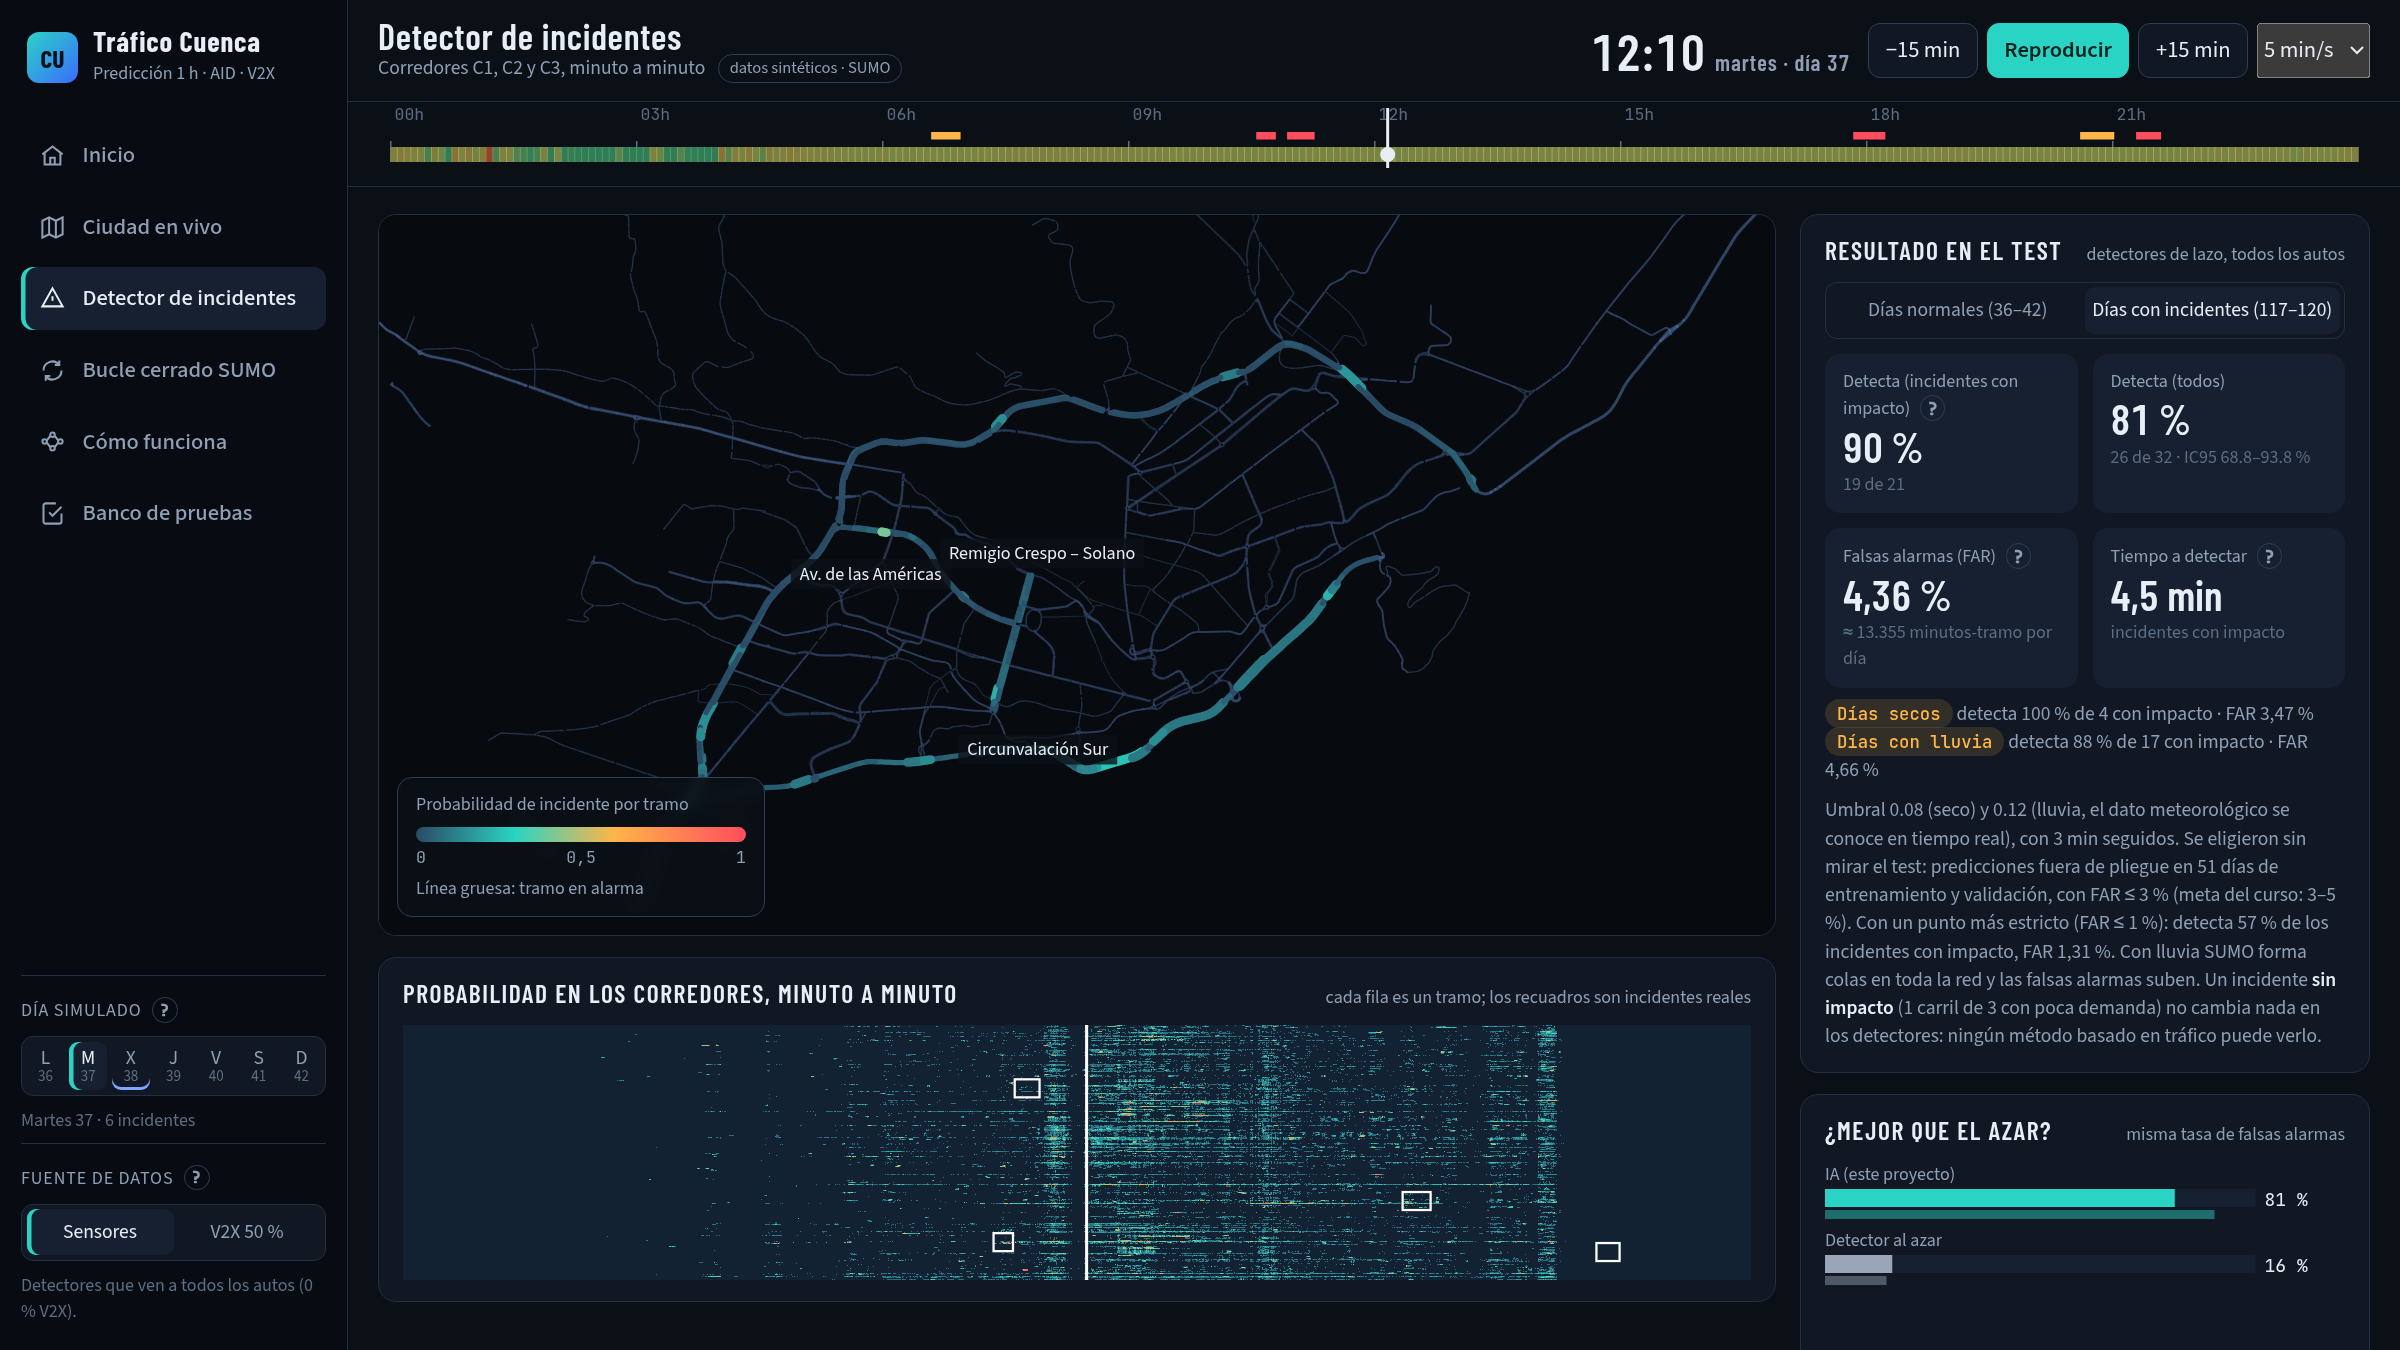
\includegraphics[width=.86\textwidth]{dash_aid_inc.png}\end{center}
Las tres avenidas vigiladas, coloreadas por la probabilidad de incidente (azul bajo, rojo alto; línea gruesa = tramo en alarma). La franja de abajo tiene una fila por tramo y una columna por minuto; los recuadros blancos son los incidentes reales. A la derecha:
\begin{itemize}[leftmargin=*]
\item El selector \textbf{Días normales / Días con incidentes} cambia el conjunto de prueba de los resultados y de la tabla de incidentes.
\item Resultados por clima (seco y lluvia), con colores: verde si las falsas alarmas están bajo 3~\%, ámbar hasta 5~\%, rojo sobre 5~\%.
\item \textbf{¿Mejor que el azar?}: la IA frente a un detector que dispara al azar con la misma cantidad de alarmas.
\item \textbf{Umbral de alarma}: al mover el control se ve cómo cambian aciertos y falsas alarmas.
\end{itemize}
\nota{El mapa y la franja son del día elegido abajo a la izquierda; los resultados de la derecha son de todo el conjunto de prueba elegido.}

\sub{Bucle cerrado SUMO}
\begin{center}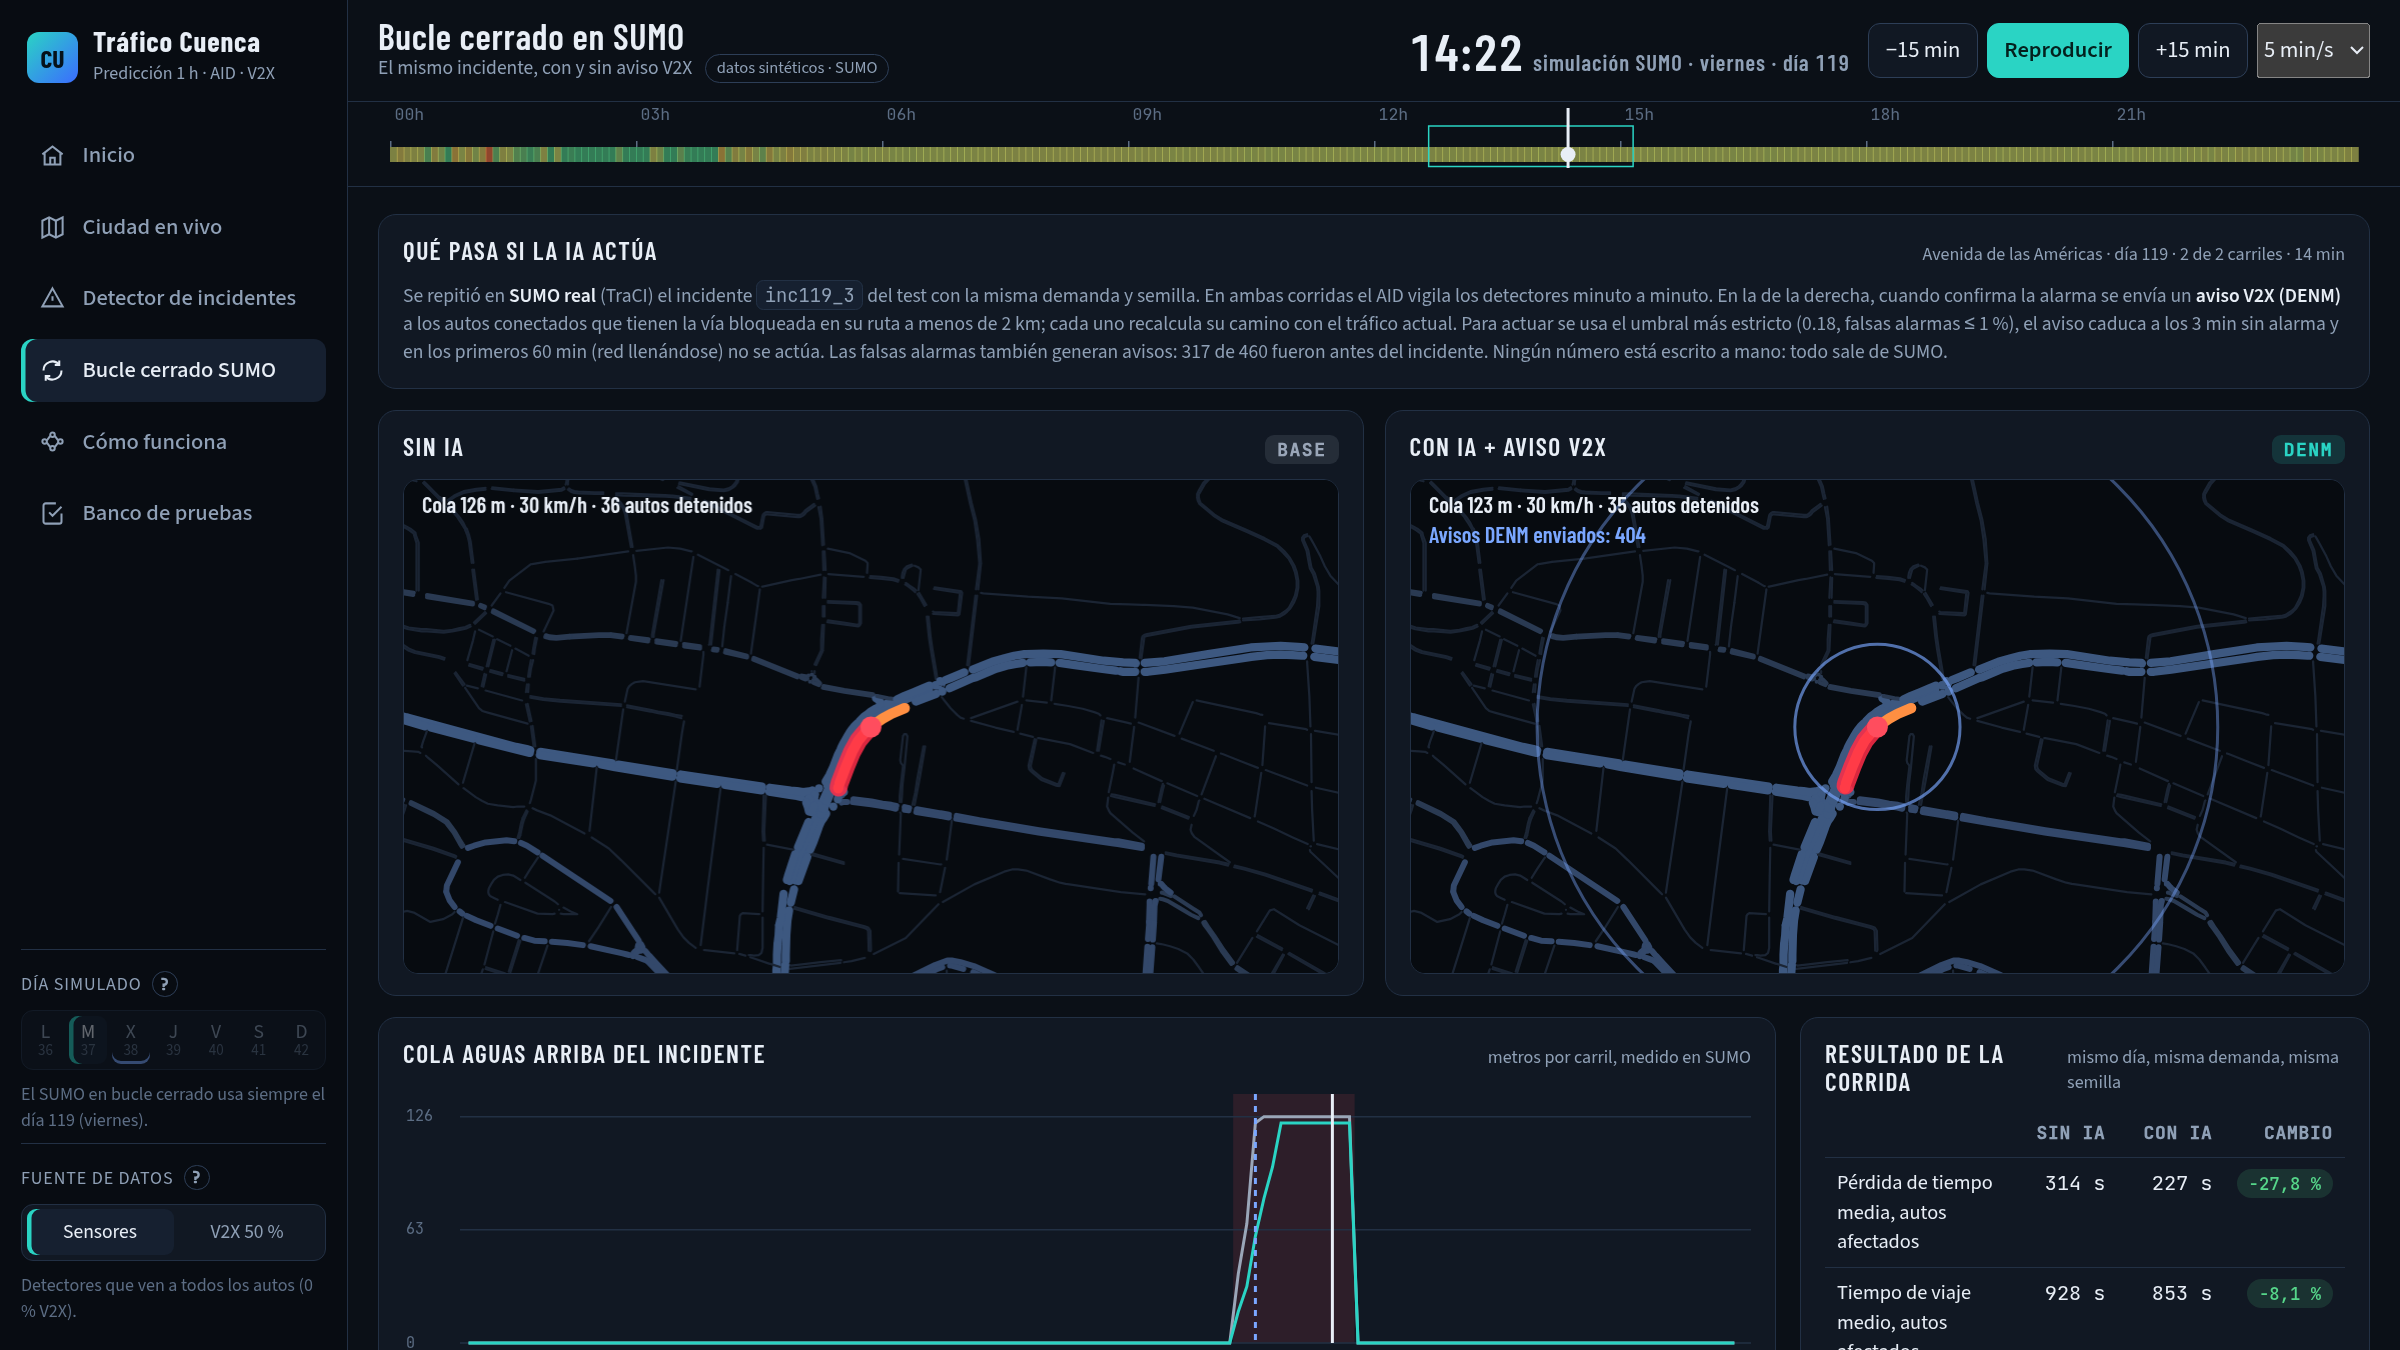
\includegraphics[width=.86\textwidth]{dash_sil.png}\end{center}
El mismo accidente (cierre total de la Av.~de las Américas, día 119, 14:10) simulado dos veces en SUMO. Izquierda: sin aviso. Derecha: con la IA y avisos V2X; los círculos azules son los avisos DENM. Debajo, la cola y la velocidad medidas en SUMO, la tabla de resultados y la línea de tiempo de lo que decidió el sistema. El texto de arriba indica cuántos avisos fueron por falsas alarmas.

\sub{Cómo funciona}
Los cinco pasos del sistema. Clic en cada tarjeta para ver qué se hizo y su gráfico.

\sub{Banco de pruebas}
Las \PruebasTotal{} verificaciones automáticas: verde pasa, rojo no pasa, con el motivo. Al lado, ``¿Mejor que la referencia?'': la IA frente a la forma simple de hacer cada cosa sin IA. Se actualiza al correr \texttt{python -m pytest pruebas/ -q} y luego \texttt{python construir\_dashboard.py}.

\seccion{4. Vistas exactas por dirección}
Agregando parámetros a la dirección se abre una vista exacta, útil para la exposición:

{\small\begin{tabular}{@{}>{\ttfamily}p{9.4cm}p{6.6cm}@{}}
localhost:8097/?t=08:00\&capa=pred\#ciudad & Predicción a las 08:00 \\
localhost:8097/?t=08:00\&capa=pred\&celda=592\#ciudad & Igual, con una celda que se congestiona \\
localhost:8097/?t=12:10\&conj=test\_incidentes\#aid & Detector con los días de incidentes \\
localhost:8097/?t=14:05\#sil & Cinco minutos antes del cierre \\
localhost:8097/?fuente=obs\#ciudad & Con datos V2X 50 \% \\
localhost:8097/?dia=38\&t=09:15\&capa=pred\#ciudad & El miércoles de lluvia \\
localhost:8097/?paso=2\#como & Paso de predicción en ``Cómo funciona'' \\
\end{tabular}}

\seccion{5. Cómo demostrarlo en la exposición}
\sub{Antes de empezar (10 minutos antes)}
\begin{enumerate}[leftmargin=*]
\item Abrir el tablero con el servidor y comprobar que carga.
\item Dejar \textbf{una pestaña} lista en \url{http://localhost:8097/?t=14:05#sil} con velocidad \textbf{2 min/s}.
\item Probar que el proyector muestra la pestaña y que se puede cambiar entre el PDF de las diapositivas y el navegador con Alt+Tab.
\item Cerrar las guías turquesa (×) para ganar espacio.
\end{enumerate}

\sub{Durante la diapositiva 13 (Karla, 1 minuto)}
\begin{enumerate}[leftmargin=*]
\item Alt+Tab al navegador. Pulsar \textbf{Reproducir}.
\item A las 14:10 aparece la cola roja en ambos mapas: ``aquí ocurre el cierre''.
\item Señalar los círculos azules del mapa derecho: ``son los avisos V2X a los autos que vienen a menos de 2 km''.
\item Pausar cerca de las 14:22. Señalar la gráfica de la cola y la tabla: ``los autos que iban al cierre pierden 28~\% menos tiempo''.
\item Alt+Tab a las diapositivas y seguir con el banco de pruebas.
\end{enumerate}

\sub{Si sobra tiempo o en las preguntas}
\begin{itemize}[leftmargin=*]
\item \textbf{Predicción:} \texttt{?t=08:00\&capa=pred\#ciudad}, alternar entre ``IA: dentro de 1 h'' y ``Real dentro de 1 h''.
\item \textbf{Detector:} \texttt{?t=12:10\#aid}, mover el control del umbral y mostrar cómo suben las falsas alarmas al bajarlo.
\item \textbf{V2X frente a sensores:} cambiar la fuente abajo a la izquierda y mostrar que la predicción casi no cambia.
\end{itemize}

\sub{Si algo falla}
\begin{tabular}{@{}p{5.8cm}p{10.4cm}@{}}
``No se pudieron cargar los datos'' & Se abrió el archivo sin servidor. Usar \texttt{servir\_dashboard.py}. \\[2pt]
``Address already in use'' & Ya hay un servidor abierto: entrar directamente a la dirección, o usar otro puerto. \\[2pt]
Letras distintas o sin estilo & No hay internet para las fuentes de Google; el tablero funciona igual. \\[2pt]
Cualquier otro problema & Quedarse en la diapositiva: la captura de la demo es el respaldo. \\
\end{tabular}

\end{document}
